%%%%%%%%%%%%%%%%%%%%%%%%%%%%%%%%%%%%%%%%%%%%%%%%%%%%%%%%%%%
\section{Theory}
\label{sec:theory}
%%%%%%%%%%%%%%%%%%%%%%%%%%%%%%%%%%%%%%%%%%%%%%%%%%%%%%%%%%%


% Theory:
%% Models (of each robot, of the global input)
%% Impossibility result
%% Controlling Mean proof
%% Controlling Variance proof (CLF)
%% A Hybrid controller using hysteresis
\subsection{Models}
Consider holonomic robots that move in the 2D plane. We want to control position and velocity of the robots. 
First, assume a noiseless system containing one robot with mass $m$.
 Our inputs are global forces $[u_x,u_y]$. We define our state vector $\mathbf{x}(t)$ as the $x$ position, $x$ velocity, $y$ position and $y$ velocity.
The state-space representation in standard form is: 
\begin{align}\label{eq:stdform}
\dot{\mathbf{x}}(t)  &=  A \mathbf{x}(t) + B \mathbf{u}(t) \\
\mathbf{y}(t) &= C \mathbf{x}(t) + D \mathbf{u}(t)\nonumber 
\end{align}

and our state space representation as:
\begin{equation}
\begin{bmatrix}
\dot{x}_1\\ 
\dot{x}_2\\
\dot{x}_3\\
\dot{x}_4
\end{bmatrix} = \begin{bmatrix}
0 & 1 & 0 & 0 \\
0 & 0 & 0 & 0\\
0 & 0 & 0 & 1\\
0 & 0 & 0 & 0
\end{bmatrix}  \begin{bmatrix}
x_1\\
x_2\\
x_3\\
x_4
\end{bmatrix} + \begin{bmatrix}
0 & 0 \\
\frac{1}{m} & 0 \\
0 & 0 \\
0 & \frac{1}{m}
\end{bmatrix}  [u_x,u_y]
\end{equation}

We want to find the number of states that we can control, which is given by the rank of the \emph{controllability matrix}
\begin{equation}
\mathcal{C} = [ B, AB, A^2B, ... , A^{n-1}B ].
\end{equation}

\begin{equation}
\textrm{Here }
\mathcal{C}=\left[
\begin{matrix} 
0 & 0\\
\frac{1}{m} & 0 \\
0 & 0 \\
0 & \frac{1}{m}
\end{matrix}
\,\middle\vert\,
\begin{matrix} 
\frac{1}{m}& 0\\
0 & 0\\
0 & \frac{1}{m}\\
0 & 0
\end{matrix}
\,\middle\vert\,
\begin{matrix} 
0 & 0\\
0 & 0 \\
0 & 0 \\
0 & 0
\end{matrix}
\,\middle\vert\,
\begin{matrix} 
0 & 0\\
0 & 0\\
0 & 0\\
0 & 0
\end{matrix}
 \right],
\end{equation}
and thus all four states are controllable.

\subsection{Independent control with multiple robots is impossible}
A single robot is fully controllable, but what happens with $n$ robots? For holonomic robots, movement in the $x$ and $y$ coordinates are independent, so for notational convenience without loss of generality we will focus only on movement in the $x$ axis. Given $n$ robots to be  controlled in the $x$ axis, there are $2n$ states: $n$ positions and $n$ velocities.
%\begin{equation}\left[ x_{1,1},x_{2,1},\ldots, x_{2n-1},x_{2n}\right]^\intercal = \left[ p_{x,1},v_{x,1},\ldots,p_{x,n},v_{x,n}\right]^\intercal. \nonumber\end{equation}
%\begin{align}
%\dot{p}_{x1} &= v_{x1}\\\nonumber
%\dot{v}_{x1} &= a_{x1}\\\nonumber
%\dot{p}_{x2} &= v_{x2}\\\nonumber
%\dot{v}_{x2} &= a_{x2}\\\nonumber
%&\vdots\\\nonumber
%\dot{p}_{xn} &= v_{xn}\\\nonumber
%\dot{v}_{xn} &= a_{xn}\nonumber
%\end{align}
Our state-space representation is:
\begin{equation}
\begin{bmatrix}
\dot{x}_{1,1}\\ 
\dot{x}_{2.1}\\
\vdots\\
\dot{x}_{1,n}\\
\dot{x}_{2,n}

\end{bmatrix} = \begin{bmatrix}
0 & 1 & \ldots & 0 & 0 \\
0 & 0 & \ldots& 0 & 0 \\
\vdots &  \vdots & \ddots & \vdots & \vdots \\
0 & 0  & \ldots & 0 & 1 \\
0 & 0 & \ldots& 0 & 0 
\end{bmatrix}  \begin{bmatrix}
x_{1,1}\\
x_{2,1}\\
\vdots \\
x_{1,n}\\
x_{2,n}
\end{bmatrix} + \begin{bmatrix}
0\\
1\\
\vdots\\
0\\
1
\end{bmatrix} u_x
\end{equation}
 However, just as with one robot, we can only control two states because $\mathcal{C}$ has rank two:
\begin{equation}
\mathcal{C}=\left[ \begin{matrix} 
0\\
1\\
\vdots\\
0\\
1
\end{matrix}
\,\middle\vert\,
  \begin{matrix} 
1\\
0\\
\vdots\\
1\\
0
\end{matrix}
\,\middle\vert\,
\begin{matrix} 
0\\
0\\
\vdots\\
0\\
0
\end{matrix}
\,\middle\vert\,
\begin{matrix} 
0\\
0\\
\vdots\\
0\\
0
\end{matrix}\,\middle\vert\,, 
\ldots \right]
\end{equation}  
\subsection{Controlling Mean Position}\label{sec:controlMeanPosition}
This means \emph{any} number of robots controlled by a global command have just two controllable states in each axis. We can not control the position of all the robots, but what states are controllable? To answer this question we create the following reduced order system that represents the average $x$ position and $x$ velocity of the $n$ robots:
\begin{align}
\begin{bmatrix}\nonumber
\dot{\bar{x}}_1 \\
\dot{\bar{x}}_2
\end{bmatrix} &= \frac{1}{n} \begin{bmatrix}
0& 1& \ldots &0& 1 \\
0& 0& \ldots &0& 0
\end{bmatrix}
\begin{bmatrix}
x_{1,1}\\
x_{2,1}\\
\vdots\\
x_{1,n}\\
x_{2,n}
\end{bmatrix} \\
&+ \frac{1}{n}\begin{bmatrix}
0& 0&  \ldots &0& 0 \\
0& 1&  \ldots &0& 1
\end{bmatrix}\begin{bmatrix} 
0\\
1\\
\vdots\\
0\\
1
\end{bmatrix} u_x
\end{align}
Thus:
\begin{equation}
\begin{bmatrix}
\dot{\bar{x}}_1 \\
\dot{\bar{x}}_2
\end{bmatrix} = \begin{bmatrix}
0& 1 \\
0& 0
\end{bmatrix}
\begin{bmatrix}
\bar{x}_1\\
\bar{x}_2
\end{bmatrix} + \begin{bmatrix} 
0\\
1
\end{bmatrix} u_x
\end{equation}

We again analyze $\mathcal{C}$:
\begin{equation}
\mathcal{C}=\left[ \begin{matrix} 
0\\
1
\end{matrix}
\,\middle\vert\,
 \begin{matrix} 
1\\
0
\end{matrix}
 \right]
\end{equation}
This matrix has rank two, and thus the average position and average velocity are controllable.


Due to symmetry, only the mean position and mean velocity are controllable. However, there are several techniques for breaking symmetry, for example by allowing independent noise sources \cite{beckerIJRR2014}, or by using obstacles \cite{Becker2013b}.

\subsection{Controlling the variance of many robots}\label{sec:VarianceControl}

The variance, $\sigma_x^2,\sigma_y^2$, of the swarm's position is computed:
\begin{align}
 \overline{x}(\mathbf{x}) = \frac{1}{n} \sum_{i=1}^n x_{1,i}, \qquad  %\nonumber \\ 
\sigma_x^2(\mathbf{x}) &= \frac{1}{n} \sum_{i=1}^n (x_{1,i} - \overline{x})^2,  \nonumber \\ 
 \overline{y}(\mathbf{x}) = \frac{1}{n} \sum_{i=1}^n x_{3,i}, \qquad  %\nonumber \\ 
\sigma_y^2(\mathbf{x}) &= \frac{1}{n} \sum_{i=1}^n (x_{3,i} - \overline{y})^2.  
%NOT 1/(N-1) because we are measuring the actual Variance, not the variance of samples drawn from a distribution
\end{align}

Controlling the variance requires being able to increase and decrease the variance.  We will list a sufficient condition for each. Both conditions are readily found at the micro and nanoscale. 
Real systems, especially at the micro scale, are affected by unmodelled dynamics. These unmodelled dynamics are dominated by Brownian noise. To model this~\eqref{eq:stdform} must be modified as follows:
\begin{align}
\dot{\mathbf{x}}(t)  &=  A \mathbf{x}(t) + B \mathbf{u}(t) + W \bm{\varepsilon}(t)\\
 \mathbf{y}(t) &= C  \mathbf{x}(t) + D  \mathbf{u}(t)\nonumber
\end{align}
where $W\bm{\varepsilon}(t)$ is a random perturbation produced by Brownian noise. Given a large free workspace, a \emph{Brownian noise} process increases the variance linearly with time.
\begin{equation}\dot{\sigma_x^2}(\mathbf{x}(t), \mathbf{u}(t) = 0)  = W \bm{\varepsilon} \end{equation}
%After some time, Gaussian distribution shapes the outline of the robots because of the Brownian noise feature:\\
%\begin{equation}
%P(x) = \frac{1}{\sigma \sqrt{2\pi } }e^{ -  \frac{\left( x - \mu  \right)^2 } {2\sigma ^2 }}
%\end{equation}
If robots with radius $r$ are in a bounded environment with sides of length $[\ell_x, \ell_y]$, the unforced variance asymptotically grows to the variance of a uniform distribution,
\begin{align}
[\sigma_x^2,\sigma_y^2] = \frac{1}{12}[ (\ell_x - 2 r)^2,(\ell_y - 2 r)^2].\label{eq:VarianceUniformDistribution}
\end{align}

 A flat obstacle can be used to decrease variance. Pushing a group of dispersed robots against a flat obstacle will decrease their variance until the minimum-variance (maximum density) packing  is reached. For large $n$, Graham and Sloan showed that the minimum-variance packing  $\sigma^2_{optimal}(n,r)$ for $n$ circles with radius $r$ is $\approx 
   \frac{\sqrt{3}}{\pi} (n r)^2\approx 0.55(n r)^2 $~\cite{graham1990penny}. 
% Sloan minimized second moment U = 1/d^2 \sum_{i=1}^{n} || P_i - P ||^2 = (\sqrt{3} n^2)/(4 \pi), where d = 2r.
% Therefore the variance is d^2 (\sqrt{3} n^2)/(4 \pi), or 4^r^2 (\sqrt{3} n^2)/(4 \pi) = r^2 (\sqrt{3} n^2)/(\pi)If we only need to reduce variance in a single axis, the variance can be reduced to zero, given sufficient space.

We will prove the origin is globally asymptotically stabilizable by using a control-Lyapunov function \cite{Lyapunov1992}.  A suitable Lyapunov function is squared variance error:
\begin{align}
\label{eq:LyapunovVariance}
V(t,\bf{x})  &= \frac{1}{2} (\sigma^2(\mathbf{x}) - \sigma^2_{goal})^2\nonumber\\
\dot{V}(t,\bf{x}) &= (\sigma^2(\mathbf{x})-\sigma^2_{goal})\dot{\sigma^2}(\mathbf{x})
\end{align}
We note here that $V(t,\mathbf{x})$ is positive definite and radially unbounded, and $V(t,\mathbf{x}) \equiv 0$ only at $\sigma^2(\mathbf{x}) = \sigma^2_{goal}$.
To make $\dot{V}(t,\mathbf{x})$ negative semi-definite, we choose
\begin{align}
u(t) &=   \begin{cases}
	 \mbox{move to wall} &\mbox{if } \sigma^2(\mathbf{x})>\sigma^2_{goal} \\ 
	 \mbox{move from wall} & \mbox{if } \sigma^2(\mathbf{x}) \le \sigma^2_{goal}.
\end{cases} 
\end{align}
 For such a $u(t)$,
 \begin{align}
\dot{\sigma^2}(\mathbf{x}) &=   \begin{cases}
	 \mbox{negative} &\mbox{if } \sigma^2(\mathbf{x})> \max(\sigma^2_{goal}, \sigma^2_{optimal}(n,r))  \\ 
	 W \epsilon & \mbox{if } \sigma^2(\mathbf{x}) \le \sigma^2_{goal},
\end{cases} 
\end{align} and thus
$\dot{V}(t,{\bf x})$ is negative definite and the variance is globally asymptotically stabilizable.% \hfill$\blacksquare$ 





\subsection{Controlling both mean and variance of many robots}

The mean and variance of the swarm cannot be controlled simultaneously, however if the dispersion due to Brownian motion is much less than the maximum controlled speed, we can adopt a hybrid, hysteresis-based controller to regulate the mean and variance shown in Alg.~\ref{alg:MeanVarianceControl}.  Such a controller normally controls the mean position according to \eqref{eq:PDcontrolPosition}, but switches to minimizing variance if the variance exceeds some $\sigma_{max}^2$.  The variance is lowered to less than $\sigma_{min}^2$, and the system returns to controlling the mean position. This is a standard technique for dealing with control objectives that evolve at different rates~\cite{Sadraddini2015,kloetzer2007temporal}, and the hysteresis avoids rapid switching between control modes. The process is illustrated in Fig.~\ref{fig:hysteresis}. 


\begin{algorithm}
\caption{Hybrid mean and variance control}\label{alg:MeanVarianceControl}
\begin{algorithmic}[1]
\Require Knowledge of swarm mean $[\bar{x},\bar{y}]$, variance $[\sigma_x^2, \sigma_y^2]$, the locations of the rectangular boundary $\{x_{min}, x_{max}, y_{min}, y_{max}\}$, and the target mean position $[x_{target},y_{target}]$.%TODO: use  \AND, \OR, \XOR, \NOT, \TO, \TRUE, \FALSE \gets
\State $flag_x \gets \FALSE$,  $flag_y \gets \FALSE$ 
\State $x_{goal} \gets  x_{target}$, $y_{goal} \gets y_{target}$
\Loop
%\State  Compute $\sigma_x^2, \sigma_y^2$

\If {$\sigma_x^2 > \sigma_{max}^2$}
\State $x_{goal}  \gets x_{min}$
\State $flag_x  \gets \TRUE$
\Else {\bf~if} {$flag_x$ \textbf{and} $\sigma_x^2 < \sigma_{min}^2$}
\State $x_{goal}  \gets  x_{target}$
\State $flag_x  \gets  \FALSE$
\EndIf

\If{$\sigma_y^2 > \sigma_{max}^2$}
\State $y_{goal}  \gets y_{min}$
\State $flag_y  \gets \TRUE$
\Else {\bf~if} {$flag_y$ \textbf{and} $\sigma_y^2 < \sigma_{min}^2$}
\State $y_{goal}  \gets  y_{target}$
\State $flag_y  \gets \FALSE$
\EndIf
\State Apply \eqref{eq:PDcontrolPosition} to move toward $[x_{goal}, y_{goal}]$
\EndLoop
\end{algorithmic}
\end{algorithm}
\begin{figure}
\centering
\begin{overpic}[scale=.3]{hysteresis.png}
\put(39,21){$\sigma^2 < \sigma^2_{min}$ }
\put(39,5){$\sigma^2 > \sigma^2_{max}$}\end{overpic}
\vspace{-1em}
\caption{\label{fig:hysteresis} Two states for controlling the mean and variance of a robot swarm.
%\vspace{-2em}
}
\end{figure}

A key challenge is to select proper values for $\sigma_{min}^2$ and $\sigma_{max}^2$.  The optimal packing variance is 
$ \sigma^2_{optimal}(n,r) = \frac{\sqrt{3}}{ \pi}  n r^2 $.  
The random packings generated by pushing our robots into corners are suboptimal, so we choose the conservative values shown in Fig.~\ref{fig:VarianceMinMaxBand}:
\begin{align}
 \sigma^2_{min} &= 2.5r+ \sigma^2_{optimal}(n,r) \nonumber\\
  \sigma^2_{max} &= 15r+ \sigma^2_{optimal}(n,r).
  \end{align}
%\sigma \approx 0.371258 n r,   \sigma_{min} = n*r*1/2, \sigma_{min} = n*r*3/2, 
%  this result was verified in http://www-math.mit.edu/~tchow/penny.pdf

\begin{figure}
\centering
\begin{overpic}[width = \columnwidth]{VarianceMinMaxBand2v2.pdf}\end{overpic}
\vspace{-1em}
\caption{\label{fig:VarianceMinMaxBand} The switching conditions for variance control are set as a function of $n$, and designed to be larger than the optimal packing density. The above plot uses robot radius $r=1/10$.
}\vspace{-1em}
\end{figure}



%what images should I show here?
%hysteresis control law, \cite{sadra2014}

\subsection{Controlling covariance using friction}
Global inputs move a swarm uniformly.  
Controlling covariance requires breaking this uniform symmetry.  A swarm inside an axis-aligned rectangular workspace can reduce variance normal to a wall by simply pushing the swarm into the boundary. Directly controlling covariance by pushing the swarm into a boundary requires changing the boundary.  An obstacle in the lower-right corner is enough to generate positive covariance.  Generating both positive and negative covariance requires additional obstacles.  Requiring special obstacle configuration also makes covariance control dependent on the local environment. 
  Instead of pushing our robots directly into a wall, this paper examines an oblique approach, by using boundaries that generate friction with the robots.  These frictional forces are  sufficient to break the symmetry caused by uniform inputs.  Robots touching a wall have a negative friction force that opposes movement along the boundary, as shown in Eq.\ \eqref{eq:frictionmodel}.  This  causes robots along the boundary to slow down compared to robots in free-space. This enables covariance control using  boundaries with arbitrary orientations. 
  
 Let the control input be a vector force $\vec{F}$ with magnitude $F$ and orientation $\theta$.  The force of friction $F_f$ is
\begin{align}
N &= F \cos(\theta) \nonumber\\
F_f &= \begin{cases}  \mu_f N, &  \mu_f N < F \sin(\theta)  \label{eq:frictionmodel} \\ 
F \sin(\theta), & \text{else} \end{cases}  \\%\sign(F \sin(\theta) ) \cdot  \max(0, | F sin\theta |- |F_f|)
F_{\text{\emph{forward}}} &=  F \sin(\theta) - F_f  \nonumber
\end{align}
 Fig.~\ref{fig:friction} shows the resultant forces on two robots when one is touching a wall. As illustrated, bot experiences different net forces although each receive the same inputs.
  For ease of analysis, the following algorithms assume $\mu_f$ is infinite and robots touching the wall are prevented from sliding along the wall.
This means that if one robot is touching the wall and another robot is free, if the control input is parallel or into the wall, the touching robot will not move. 
The next section shows how a system with friction model \eqref{eq:frictionmodel} and two walls are sufficient to arbitrarily position two robots. 
\begin{figure}[h]
\begin{center}
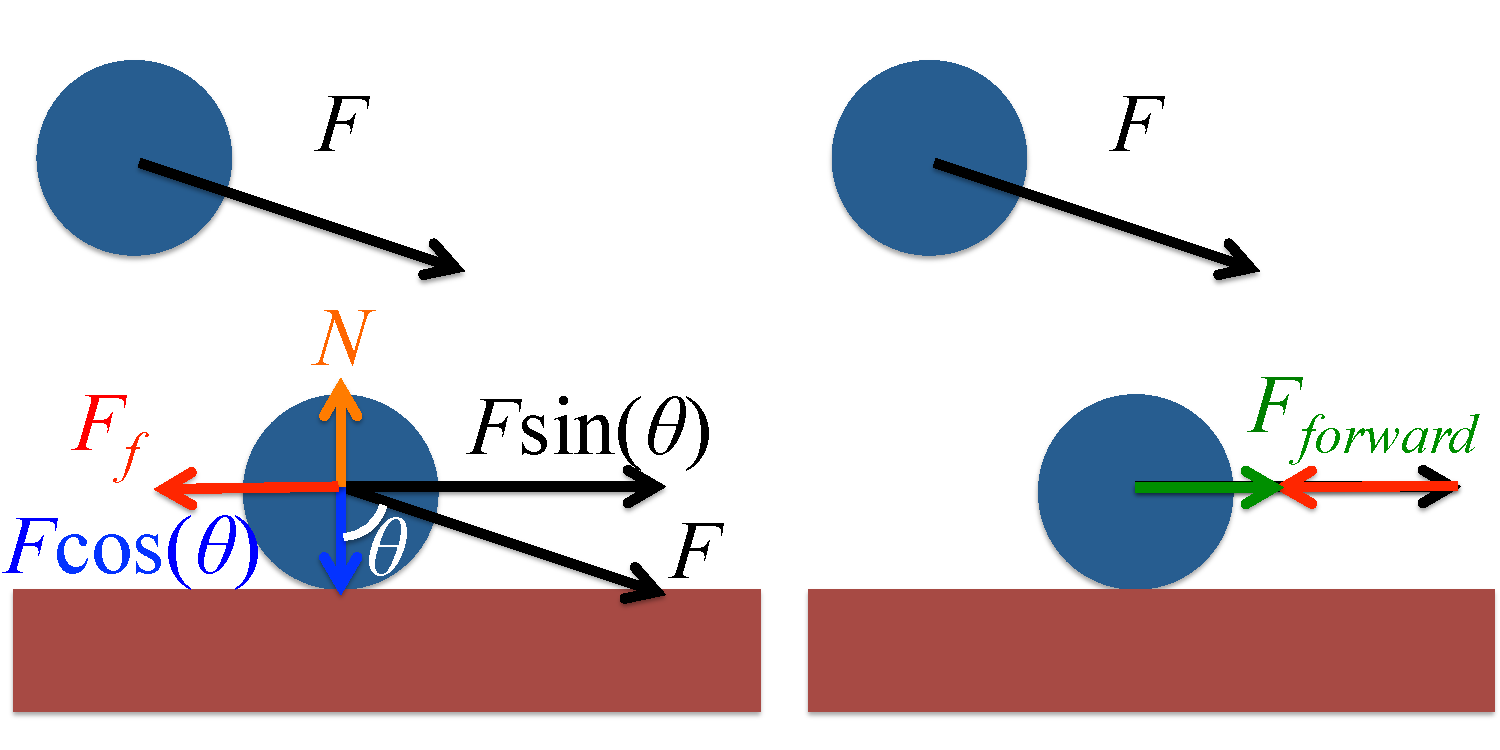
\includegraphics[width=\columnwidth]{friction.pdf} 
\caption{Wall friction reduces the force for going forward $F_{\text{\emph{forward}}}$ on a robot near a wall, but not for a free robot.}
\label{fig:friction}
\end{center}
\end{figure} 




\section{Position control of $2$ robots using wall friction}\label{sec:PostionControl2Robots}
This section describes an algorithm for positioning two robots and introduces concepts that will be used for multi-robot positioning.
%Although the generalization of the proposed positioning algorithm in here is rather straightforward for multi robot systems, for the sake of simplicity we describe the algorithm designed for two robots. 
As we can see in Alg.~\ref{alg:PosControl2Robots}, assume two robots are initialized at $s_1$ and $s_2$ with corresponding goal destinations $e_1$ and $e_2$. 
Denote the current positions of the robots  $r_1$ and $r_2$. 
Let the subscripts $x$ and $y$ denote the $x$ and $y$ coordinates, i.e., $s_{1x}$ and $s_{1y}$ denote the $x$ and $y$ locations of $s_1$. 
The algorithm assigns a global control input at every instance.
 As a result, our goal is to adjust 
 $\Delta r_x = r_{2x}-r_{1x}$ from $\Delta s_x = s_{2x}-s_{1x}$ to $\Delta e_x = e_{2x}-e_{1x}$ and similarly adjust 
 $\Delta r_y = r_{2y}-r_{1y}$ from $\Delta s_y = s_{2y}-s_{1y}$ to $\Delta e_y = e_{2y}-e_{1y}$ with one global input at every instance. 
 The key to the algorithm is the position-dependent friction model \eqref{eq:frictionmodel}.
 %employing the assumption we have made earlier about the walls' friction. 

Our algorithm uses a divide and conquer method to solve the positioning problem. 
It finds the final position of the robots in two steps: (i) First, $|\Delta r_x - \Delta e_x |$ is reduced to zero while  $\Delta r_y$ is kept constant in Alg.~\ref{alg:XControl}. 
(ii) Having fixed $\Delta r_x$ to $\Delta e_x$ as desired, the  algorithm next keeps $\Delta r_x$ constant and adjusts $\Delta r_y$ to $\Delta e_y$, as desired in Alg..~\ref{alg:YControl}. 
Though steps (i) and (ii) are similar from an algorithmic point of view, the following subsections describe the process in detail. 

\subsection{Step (i): Fixing $\Delta r_x$}
\label{theory:step1}
\begin{itemize}
\item Define $e'_1=(e_{1x},s_{1y})$ and $e'_2=(e_{2x},s_{2y})$. Our goal for defining $e'_1$ and $e'_2$ is to understand the direction to which robots should move in order to adjust $\Delta r_x$. Let $e'_{\rm{top}} = \arg \max_i e'_{iy}$ and $e'_{\rm{bottom}} = \arg \min_i e'_{iy}$. Now if $e'_{\rm{top},x}-e'_{\rm{bottom},x}>0$, then the global input to both robots would be toward left direction and if $e'_{\rm{top},x}-e'_{\rm{bottom},x}<0$, then the global input to both robots would be toward right direction. The two robots continue their horizontal path until one of them reaches the $\epsilon$-neighborhood of one of the left or right walls.
\item At this step, let $y_{\min} = \min_i r_{iy}$, i.e., $y_{\min}$ is the minimum height of the two robots. We move both robots downward by the amount of $y_{\min}$ such that one of the robots would touch the bottom wall and hence friction force will not let that robot to move left or right.
\item The fact that the friction force of the bottom wall would not let the lower robot to move right or left will let the other robot to move to right and left freely to adjust $\Delta r_x $ according to $\Delta e_x$.
\item Finally, even if with the free move of the upper robot $\Delta r_x$ is not set to the $\Delta e_x$, we can run the Step (i) (as described in the previous paragraphs) again to adjust the $\Delta r_x$. It is easy to show that it is guaranteed that we can adjust $\Delta r_x$ to $\Delta e_x$ in only two iterations.
\end{itemize}

\subsection{Step (ii): Fixing $\Delta r_y$}
Now that we have adjusted the difference in robots' positions along one axis, we focus to do the same on the other axis as well. Therefore, similar to Section \ref{theory:step1}, we employ the following steps:
\begin{itemize}
\item Let $s'_1$ and $s'_2$ be the points we derived at the end of the steps in Section \ref{theory:step1}. 
\item Define $e''_1=(s'_{1x},e_{1y})$ and $e''_2=(s'_{2x},e_{2y})$. We define $e''_1$ and $e''_2$ to understand the direction to which robots should move in order to adjust $\Delta r_y$. Let $e''_{\rm{right}} = \arg \max_i e''_{ix}$ and $e''_{\rm{left}} = \arg \min_i e'_{ix}$. Now if $e''_{\rm{right},y}-e''_{\rm{left},y}>0$, then the global input to both robots would be toward down direction and if $e''_{\rm{right},y}-e''_{\rm{left},y}<0$, then the global input to both robots would be toward up direction. The two robots continue their vertical path until one of them reaches the $\epsilon$-neighborhood of one of the top or bottom walls.
\item At this step, let $x_{\min} = \min_i r_{ix}$, i.e., $x_{\min}$ is the minimum distance of the two robots from the origin along the $x$-axis. We move both robots to the left by the amount of $x_{\min}$ such that one of the robots would touch the left wall and hence friction force will not let that robot to move up or down.
\item The fact that the friction force of the left wall would not let one of the robots to move up or down will let the other robot to move to up or down freely to adjust $\Delta r_y $ according to $\Delta e_y$.
\item Finally, even if with the free move of the robot which is not touching the wall  $\Delta r_y$ is not set to the $\Delta e_y$, we can run the Step (i) (as described in the previous paragraphs) again to adjust the $\Delta r_y$. It is easy to show that it is guaranteed that we can adjust $\Delta r_y$ to $\Delta e_y$ in only two iterations.
\end{itemize}
Once $\Delta r_x$ and $\Delta r_y$ are set to $\Delta e_x$ and $\Delta e_y$, we can use global input to easily move both robots from $r_1$ and $r_2$ toward $e_1$ and $e_2$. 


\begin{algorithm}
\caption{WallFrictionArrange2Robots($s_1,s_2,e_1,e_2,L$)}\label{alg:PosControl2Robots}
\begin{algorithmic}[1]
\Require 
Knowledge of starting $(s_1,s_2)$ and ending $(e_1,e_2)$ positions of  two robots. 
$(0,0)$ is bottom corner, $s_1$ is rightmost robot, 
 $L$ is length of the walls. 
 Current position of the robots are $(r_1,r_2)$.

\State ($r_1,r_2$) = GenerateDesired$x$-spacing($s_1,s_2,e_1,e_2,L$)
\State GenerateDesired$y$-spacing($r_1,r_2,e_1,e_2,L$)

\end{algorithmic}
\end{algorithm}


\begin{algorithm}
\caption{GenerateDesired$x$-spacing($s_1,s_2,e_1,e_2,L$)}\label{alg:XControl}
\begin{algorithmic}[1]
\Require Knowledge of starting $(s_1,s_2)$ and ending $(e_1,e_2)$ positions of  two robots. 
$(0,0)$ is bottom corner, $s_1$ is topmost robot, 
 $L$ is length of the walls. Current robot positions are $(r_1,r_2)$.
\Ensure   $ r_{1y} - r_{2y}  \equiv s_{1y} - s_{2y} $   %$\Delta y(t) \equiv \Delta y(0)$ 
\State $\epsilon \gets $ small number
\State $ \Delta s_x  \gets s_{1x} - s_{2x} $
\State $ \Delta e_x \gets e_{1x} - e_{2x} $
\State $ r_1 \gets s_1$, $ r_2 \gets s_2$
\If {$\Delta e_x < 0 $ }
\State $ m \gets ( L-\epsilon-\max( r_{1x},r_{2x}) ,0)   $ \Comment{Move to right wall}
\Else 
\State  $ m \gets ( \epsilon-\min( r_{1x},r_{2x}),0 )    $ \Comment{Move to left wall}
\EndIf
\State $m  \gets  m + (0, -\min( r_{1y},r_{2y} ))$ \Comment{Move to bottom}
\State $ r_1 \gets r_1+m$, $ r_2 \gets r_2+m$ \Comment{Apply move}
\If {$\Delta e_x - (r_{1x} - r_{2x} ) > 0 $}
\State $ m \gets (\min(|\Delta e_x - \Delta s_x |, L- r_{1x}), 0)$  \Comment{Move right}
\Else
\State $ m \gets (-\min(|\Delta e_x - \Delta s_x |, r_{1x}), 0)$\Comment{Move left}
\EndIf 
\State $m  \gets  m + (0, \epsilon)$ \Comment{Move up}
\State $ r_1 \gets r_1+m$, $ r_2 \gets r_2+m$ \Comment{Apply move}
\State $\Delta r_x = r_{1x} - r_{2x}$
\If {$\Delta r_x \equiv \Delta e_x$} 
%\State   $ m \gets (e_{1x}-r_{1x}, e_{1y}-r_{1y})$
%\State $ r_1 \gets r_1+m$, $ r_2 \gets r_2+m$ \Comment{Apply move}
\State  \Return $(r_1,r_2)$
\Else   
\State \Return GenerateDesired$x$-spacing($r_1,r_2,e_1,e_2,L$)
\EndIf
\end{algorithmic}
\end{algorithm}

\begin{algorithm}
\caption{GenerateDesired$y$-spacing($s_1,s_2,e_1,e_2,L$)}\label{alg:YControl}
\begin{algorithmic}[1]
\Require Knowledge of starting $(s_1,s_2)$ and ending $(e_1,e_2)$ positions of  two robots. 
$(0,0)$ is bottom corner, $s_1$ is rightmost robot, 
 $L$ is length of the walls. Current position of the robots are $(r_1,r_2)$.
\Ensure   $ r_{1x} - r_{2x}  \equiv s_{1x} - s_{2x} $   %$\Delta y(t) \equiv \Delta y(0)$ 
\State $ \Delta s_y  \gets s_{1y} - s_{2y} $
\State $ \Delta e_y \gets e_{1y} - e_{2y} $
\State $ r_1 \gets s_1$, $ r_2 \gets s_2$
\If {$\Delta e_y < 0 $ }
\State $ m \gets ( L-\max( r_{1y},r_{2y}) ,0)   $ \Comment{Move to top wall}
\Else 
\State  $ m \gets ( -\min( r_{1y},r_{2y}),0 )    $ \Comment{Move to bottom wall}
\EndIf
\State $m  \gets  m + (0, -\min( r_{1x},r_{2x} ))$ \Comment{Move to left}
\State $ r_1 \gets r_1+m$, $ r_2 \gets r_2+m$ \Comment{Apply move}
\If {$\Delta e_y - (r_{1y} - r_{2y} ) > 0 $}
\State $ m \gets (\min(|\Delta e_y - \Delta s_y |, L- r_{1y}), 0)$  \Comment{Move top}
\Else
\State $ m \gets (-\min(|\Delta e_y - \Delta s_y |, r_{1y}), 0)$\Comment{Move bottom}
\EndIf 
\State $m  \gets  m + (0, \epsilon)$ \Comment{Move right}
\State $ r_1 \gets r_1+m$, $ r_2 \gets r_2+m$ \Comment{Apply move}
\State $\Delta r_y = r_{1y} - r_{2y}$
\If {$\Delta r_y \equiv \Delta e_y$} 
\State   $ m \gets (e_{1x}-r_{1x}, e_{1y}-r_{1y})$
\State $ r_1 \gets r_1+m$, $ r_2 \gets r_2+m$ \Comment{Apply move}
\State  \Return $(r_1,r_2)$
\Else   
\State \Return GenerateDesired$y$-spacing($r_1,r_2,e_1,e_2,L$)
\EndIf
\end{algorithmic}
\end{algorithm}









